\begin{figure}[hp!]
\centering
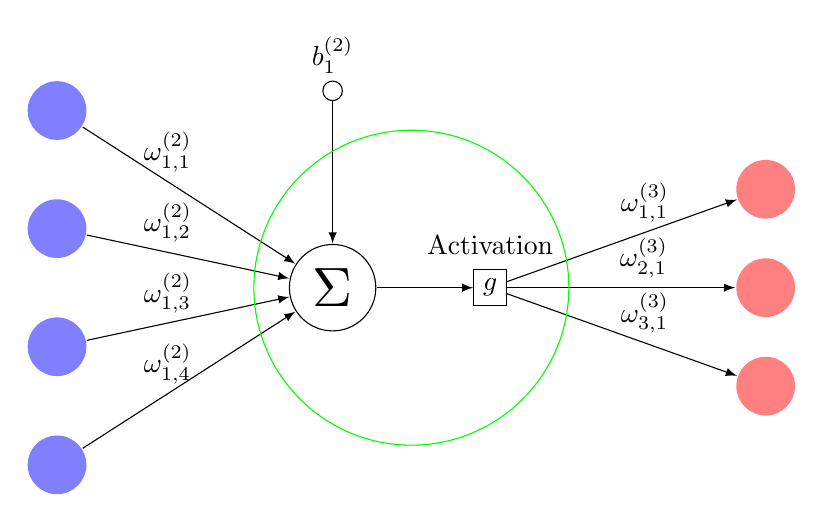
\begin{tikzpicture}[>=latex]
\path
(0,0)     node[circle,draw,scale=2,inner sep=2pt] (S) {$\Sigma$}
+(90:2.5) node[circle,draw,inner sep=2.5pt] (b) {}
          node[above=1mm] {$b_1^{(2)}$}
+(-3.5,2.25)  node[circle,scale=2.25,fill=blue!50]  (x1) {} %{$T_{2m}$}
+(-3.5,0.75)  node[circle,scale=2.25,fill=blue!50]  (x2) {} %{$q_v$}
+(-3.5,-0.75) node[circle,scale=2.25,fill=blue!50]  (x3) {} %{$RH$}
+(-3.5,-2.25) node[circle,scale=2.25,fill=blue!50]  (x4) {} %{$p_s$}
(2,0)    node[draw] (g) {$g$} node[above=3mm]{Activation}

+(3.5,1.25)  node[circle,scale=2.25,fill=red!50]  (y1) {}
+(3.5,0)  node[circle,scale=2.25,fill=red!50]  (y3) {}
+(3.5,-1.25) node[circle,scale=2.25,fill=red!50]  (y2) {};

\draw[->] (S)--(g);
\draw[->] (b)--(S);
\draw[->] (g)--(y1) node[pos=.6,above]{$\omega_{1,1}^{(3)}$};
\draw[->] (g)--(y2) node[pos=.6,above]{$\omega_{3,1}^{(3)}$};
\draw[->] (g)--(y3) node[pos=.6,above]{$\omega_{2,1}^{(3)}$};

\draw[->] (x1)--(S) node[pos=.4,above]{$\omega_{1,1}^{(2)}$};
\draw[->] (x2)--(S) node[pos=.4,above]{$\omega_{1,2}^{(2)}$};
\draw[->] (x3)--(S) node[pos=.4,above]{$\omega_{1,3}^{(2)}$};
\draw[->] (x4)--(S) node[pos=.4,above]{$\omega_{1,4}^{(2)}$};
\draw[green] (1,0) circle(2);
\end{tikzpicture}

\caption{Computational graph showing the components participating in the activation of a neuron in the hidden layer. This example shows a 2-layer neural network with four input nodes and three output nodes. The number of nodes in the hidden layer doesn't affect the activation of the other nodes \textcolor{red}{input and output nodes?}. The sum of the weighted input and bias is passed to the activation function \textcolor{red}{
inside the hidden layers?}. Producing the activation of the neuron. This is again passed to the output neurons. Skissen bygger videre på eksempelet fra \textcolor{red}{Modiefied skecth based on} \href{https://tex.stackexchange.com/questions/505741/architecture-neural-network-with-weights}{https://tex.stackexchange.com/questions/505741/architecture-neural-network-with-weights}. }
\label{fig:activation_one_node}
\end{figure}